\documentclass[14px]{article}
\usepackage{xeCJK}
\usepackage[frenchb]{babel}
\usepackage[T1]{fontenc}
\usepackage[utf8]{inputenc}
\usepackage{textcomp}
\usepackage{amssymb}
\usepackage[ruled,longend]{algorithm2e}
\usepackage{amsmath}
\usepackage{latexsym}
\usepackage{fancyhdr}
\usepackage{geometry}
\usepackage{setspace}

% Image
\usepackage{graphicx}
\usepackage{subfigure}
\usepackage{caption}
\usepackage{float}
% wrap
\usepackage{wrapfig}
\usepackage[colorlinks,linkcolor=blue]{hyperref}

\renewcommand{\baselinestretch}{1.2}

\begin{document}
	\setlength{\parindent}{0pt}
	\begin{titlepage}
		
		\begin{center}
			% Upper part of the page
			
\includegraphics[width=0.35\textwidth]{logo.png}\\[1cm]
			
			\textsc{\Large Rapport du projet 2 de DAAR}\\[0.5cm]
			
			% Title
			
			{ \huge \bfseries Decentralized Wikipedia}\\[0.4cm]
			
			% Author and supervisor
			\begin{minipage}{0.4\textwidth}
				\begin{flushleft} \large
					\emph{Rédacteurs:}\\
					Qiwei \textsc{XIAN}\\
					Mehdi-Nassim \textsc{KHODJA}\\
					Adel EL AMRAOUI
				\end{flushleft}
			\end{minipage}
			\begin{minipage}{0.4\textwidth}
				\begin{flushright} \large
					\emph{Professeur:} \\
					Prof.\textsc{Guillaume-Hivert}
				\end{flushright}
			\end{minipage}
			
			\vfill
			% Bottom of the page
			{\large \today}
		\end{center}
		
	\end{titlepage}
	\clearpage
	
	\tableofcontents
	\thispagestyle{empty}
	\clearpage
	
	\pagestyle{fancy}
	\lhead{Préface}
	\rhead{\thepage}
	\fancyfoot{}
	
	\section{Préface}
	\subsection{Objectif}
	L'objectif du projet est de réaliser un wikipédia décentralisé. Tous les utilisateurs ont le droit d'ajouter des articles dans ce wikipédia, ainsi que de consulter et de modifier les articles existants.
	\subsection{Techninologies utilisées}
	\begin{enumerate}
		\item React.js hook: Visualiser les résultats de nos fonctions back-end de recherche, d'ajout et de modification des articles.
		\item API Web3: Faire intéragir notre page web avec nos smart contracts. Cette API nous permet d'appeler les différentes fonctions  qu'on a définit comme smart contract dans Wikipedia.sol.
		\item Smart contract: Définir les classes qu'on veut stocker sur la blockchain ainsi que leurs opérations. 
		\item Ganache: Construire une blockchain locale. Ganache nous propose un environnement pour installer les smart contracts et générer des comptes virtuels.
		\item Metamask: Plugin de chrome. Lorsque l'utilisateur envoie une transaction, Metamask affiche une fenêtre qui permet de signer la transaction.
	\end{enumerate}
	
	\clearpage
	\pagestyle{fancy}
	\lhead{Architecture}
	\rhead{\thepage}
	\fancyfoot{}
	\section{Architecture du projet}
	\subsection{Structure de l'application}
		\begin{enumerate}
		\item contracts/Wikipedia.sol: Définition des méthodes de recherche, modification et d'ajout d'article dans notre wikipedia décentralisé.
		\item src/services/Ethereum.js: Tous les appels des APIs web3 sont encapsulés dans ce fichier. Il permet les interactions entre notre partie front-end et nos smart contracts.
		\item src/App.js: C'est la partie front-end de l'application, elle permet de générer dynamiquement le contenu des pages en utilisant des appels asynchrones.
		\end{enumerate}
	
	
	\clearpage
	\pagestyle{fancy}
	\lhead{Fonctionnalités l'ajout}
	\rhead{\thepage}
	\fancyfoot{}
	\section{Fonctionnalités de l'application}
	\subsection{Ajouter un article}
	Pour ajouter un article il est nécessaire de spécifier un id entier et un contenu sous la forme d'une chaîne de caractères puis il faut cliquer sur "submit". Submit va faire appel à la fonction addArticle de Ethereum.js pour utiliser notre smart contract addArticle définit dans wikipedia.sol.
	\begin{figure}[H]
		\begin{minipage}[H]{0.7\linewidth}
			\centering
			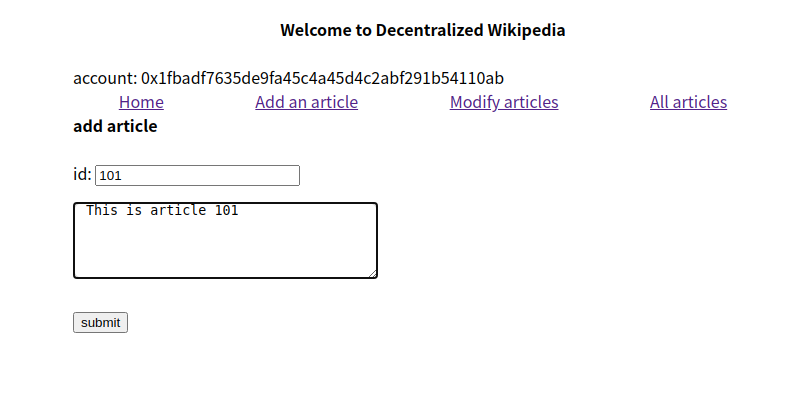
\includegraphics[width=\textwidth]{Add01.png}\\
			\caption{Saisir ID et l'article}
			\label{img1}
		\end{minipage}
		\begin{minipage}[H]{0.3\linewidth}
			\centering
			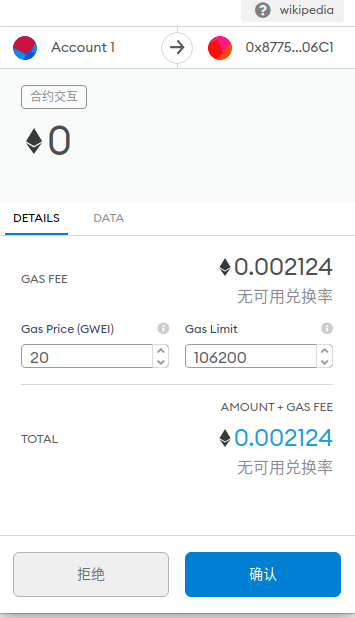
\includegraphics[width=\textwidth]{Add2.png}
			\caption{Signer la transaction}
			\label{img2}
		\end{minipage}
		\begin{minipage}[H]{0.4\linewidth}
			\centering
			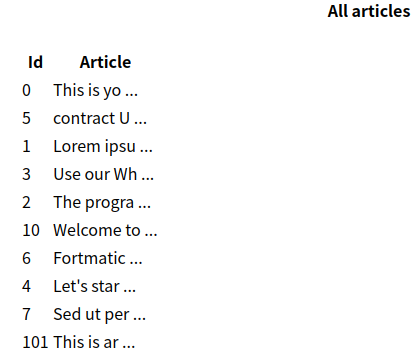
\includegraphics[width=\textwidth]{Add03.png}
			\caption{Le résultat de l'addition}
			\label{img2}
		\end{minipage}
	\end{figure}
	
	\clearpage
    \pagestyle{fancy}
	\lhead{Fonctionnalités la consultation}
	\rhead{\thepage}
	\fancyfoot{}
	\subsection{Consulter la liste des articles}
	Chaque article est identifié par un Id sous la forme d'un entier et possède un contenu représenté par une chaîne de caractères.
	La liste des articles est récupérée en cliquant sur "All articles".  All articles va faire un appel asynchrone à la fonction  getAllArticles de Ethereum.js pour afficher la liste des articles.
	\begin{figure}[H]
		\begin{minipage}[H]{\linewidth}
			\centering
			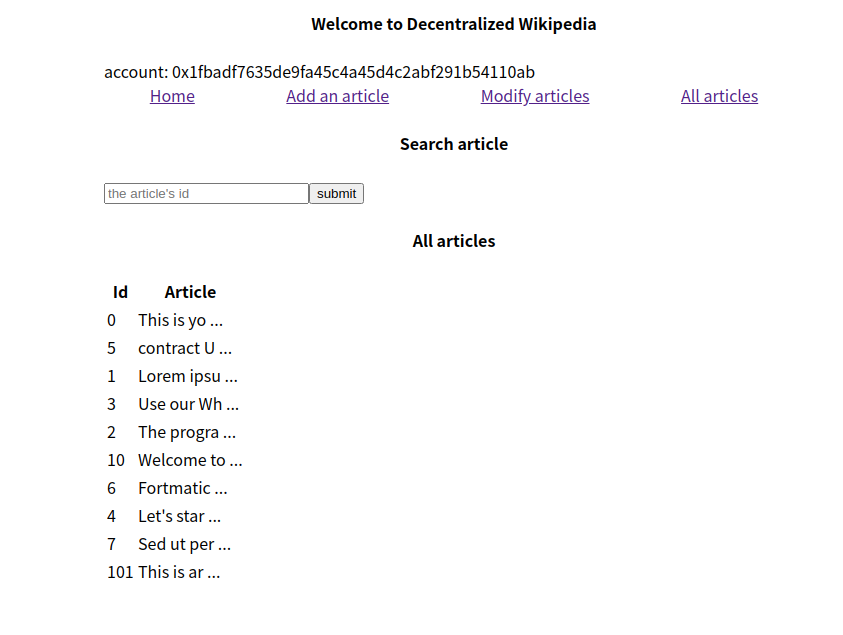
\includegraphics[width=\textwidth]{Consulter01.png}\\
			\caption{Afficher tous les articles existants}
			\label{img1}
		\end{minipage}
	\end{figure}
	
	\clearpage
	\pagestyle{fancy}
	\lhead{Fonctionnalités la recherche}
	\rhead{\thepage}
	\fancyfoot{}
	
	\subsection{Rechercher un article}
	Pour rechercher un article on spécifie l'Id de l'article dans la barre de recherche puis on clique sur submit. Cette action va appeler la fonction getArticleById de Ethereum.js et va afficher le contenu de l'article qui possède l'Id spécifiée. Dans le cas où l'article n'existe pas elle affichera un contenu vide.
	\begin{figure}[H]
		\begin{minipage}[H]{\linewidth}
			\centering
			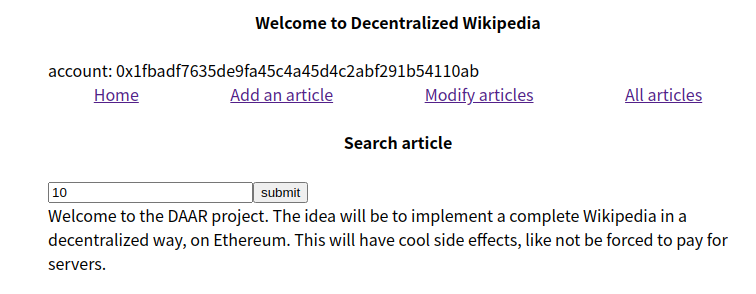
\includegraphics[width=\textwidth]{Search01.png}\\
			\caption{Chercher l'article par ID}
			\label{img1}
		\end{minipage}
	\end{figure}
	
	\clearpage
	\pagestyle{fancy}
	\lhead{Fonctionnalités la modification}
	\rhead{\thepage}
	\fancyfoot{}
	
	\subsection{Modification l'article}
	Pour modifier un article il suffit de cliquer sur "Modify articles" puis de saisir l'id de l'article et le nouveau contenu sous la forme d'une chaîne de caractères puis submit. Cela aura pour effet d'appeler de manière asynchrone la fonction modifyArticle de Ethereum.js qui va à son tour appeler le contrat modifyContent de Wikipedia.sol en précisant comme argument l'index de l'article correspondant et le nouveau contenu. La modification d'un article dont l'id n'existe pas n'aura donc aucun effet.
		\begin{figure}[H]
		\begin{minipage}[H]{0.7\linewidth}
			\centering
			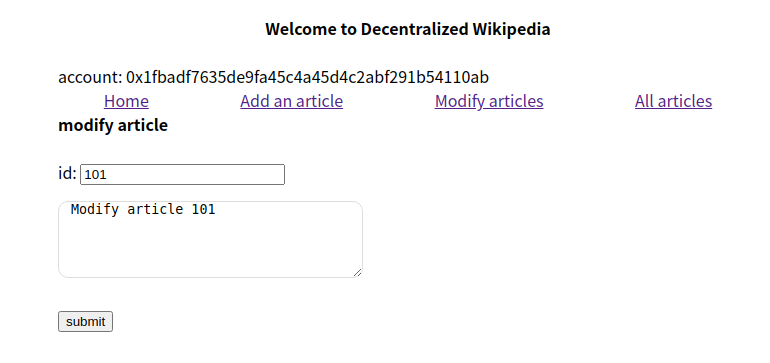
\includegraphics[width=\textwidth]{Modify01.png}\\
			\caption{Saisir ID et le nouvel article}
			\label{img1}
		\end{minipage}
		\begin{minipage}[H]{0.3\linewidth}
			\centering
			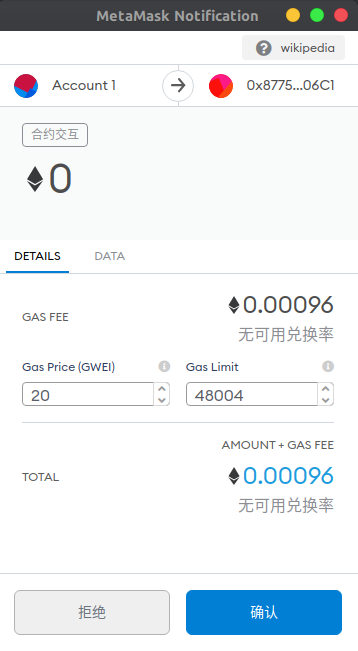
\includegraphics[width=\textwidth]{Modify02.png}
			\caption{Signer la transaction}
			\label{img2}
		\end{minipage}
		\begin{minipage}[H]{0.7\linewidth}
			\centering
			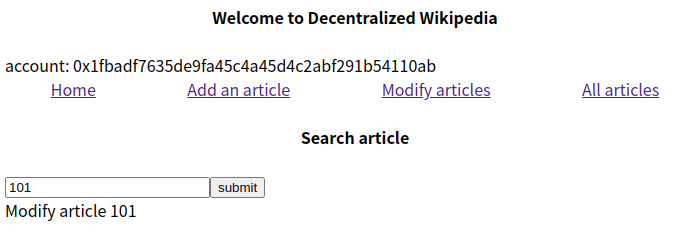
\includegraphics[width=\textwidth]{Modify03.png}
			\caption{Le résultat de la modification}
			\label{img2}
		\end{minipage}
	\end{figure}

\clearpage
\pagestyle{fancy}	
\lhead{Difficultés techniques}
\rhead{\thepage}
\fancyfoot{}
\section{Difficultés techniques rencontrées}
Pour les fonctionnalités d'ajout d'article et de modification d'article, parfois l'appel ne produit pas directement de demande de signature avec MetaMask ce qui nous contraint à recommencer une nouvelle fois la demande. En analysant l'exécution, on remarque pourtant que la fonction demandée est bien appelée malgré le fait que MetaMask n'envoie pas la demande de signature.
	
    \begin{figure}[H]
		\begin{minipage}[H]{\linewidth}
			\centering
			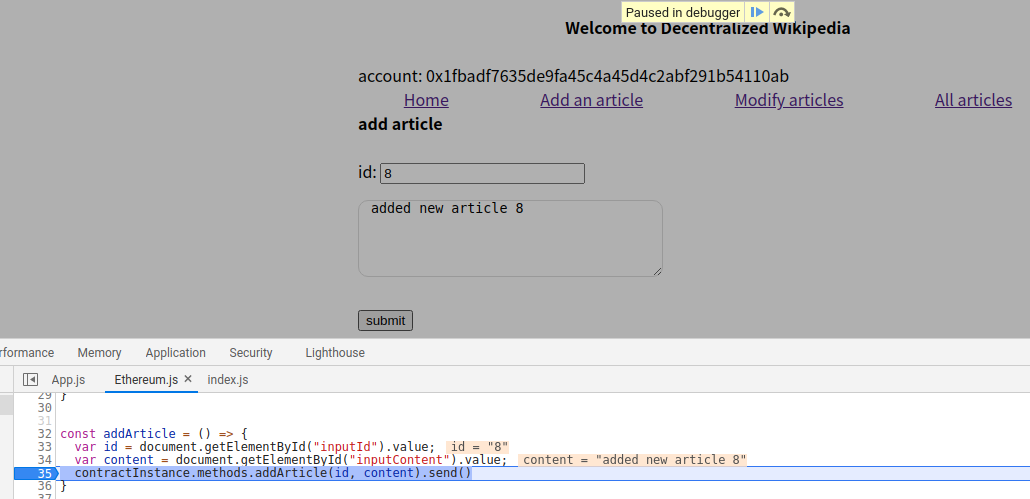
\includegraphics[width=\textwidth]{bug.png}\\
			\caption{La fonction de demande est bien appelée}
			\label{img1}
		\end{minipage}
	\end{figure}
	
	
\end{document}
